\documentclass[10pt]{article}
\usepackage[margin=0.65in]{geometry}
\usepackage{graphicx,hyperref,booktabs}
\hypersetup{colorlinks=true,urlcolor=blue}
\setlength{\parindent}{0pt}\setlength{\parskip}{5pt}
\begin{document}
\begin{center}\Large Native ECBench online boundary\\
\normalsize Software correction and pre-data continuation -- 2026-11-04\end{center}
Target subgroup validation now begins the native online interval after initial
reusable preparation. The previous ordering charged its scalar multiplication
to setup. Source/selector/width and partial collection share the corrected
boundary. Later retries and all internal replay stay inside online.
\texttt{[pcc:unverified]}

The original-ordering regression fails on one scalar call left in setup;
the corrected control requires zero there and one in target validation, and
checks the full cold/online partition. Producer logs report 121 native tests
in crypto and 98 in cryptanalysis, with format, strict lint and Rust 1.78
all-target checks. These are local development observations, without an
independent signed verdict: PCC-20261104-9bb71e and PCC-20261104-0f6851.
\texttt{[pcc:unverified]}

\begin{center}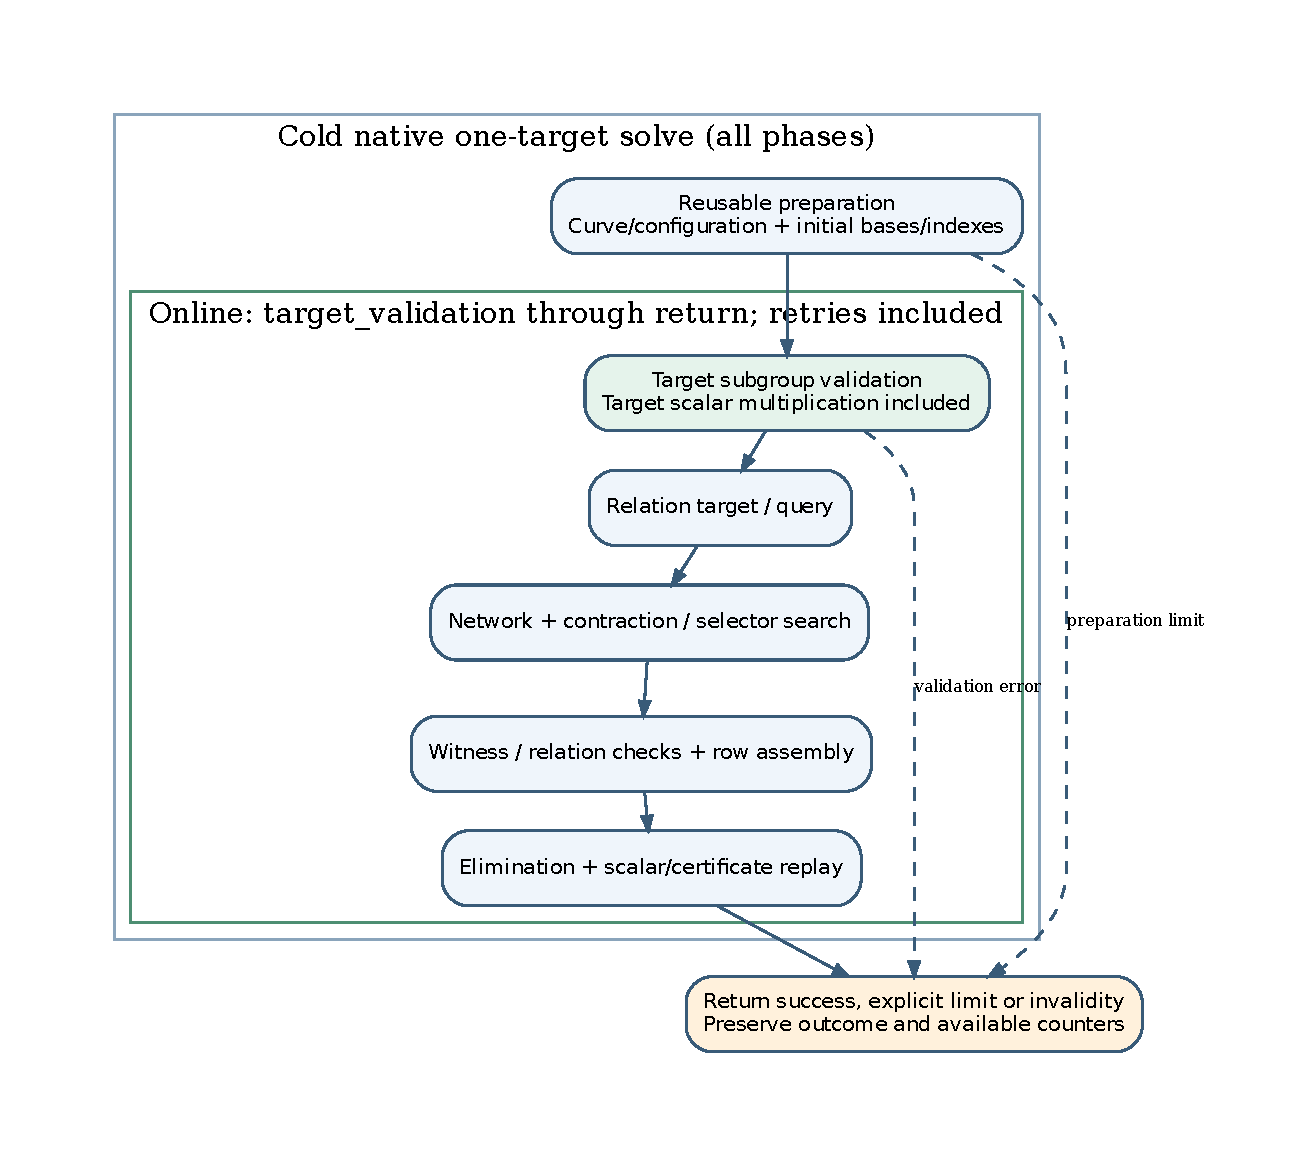
\includegraphics[height=4.65in]{online-boundary.pdf}\end{center}

The original 1,728-attempt panel and frozen v1/v2 remain preserved. A new
pre-data amendment binds current source and accounting. Current budget headroom,
source publication, fresh S3 readback and authenticated exact-image admission
precede any cloud build/measurement as applicable. Local test time is not the
study's measurement. Unpriced arithmetic and observer overhead remain disclosed.
\texttt{[pcc:unverified]}

\textbf{Sources and custody.} README.md links the pinned reduction, review
thread, exact source manifests, original failure and corrected receipts,
ECBench contract and current cost/PCC/benchmark-record rules. Editable diagram
and report sources are beside this PDF. No runtime-gain result is reported.
\end{document}
